\section{Platforms}
The suitable platforms for this project is examined in the following section. These platforms are capable of running application code and reading or writing to pins. These pins can contains components such as sensors, actuators and so on.

\subsection{Arduino}\label{sec:arduino}
Arduino is an open source platform, which makes the software and hardware documentation available to the public. The name "Arduino" covers both the software platform and the range of hardware platforms with boards of different sizes, from the smaller Arduino Nano up to the Arduino Mega. One of the more popular Arduino boards is the Arduino Uno which is a medium board, often used for starters \cite{arduinouno}.

Arduino boards have input and output ports, enabling them to read and write to sensors, actuators and other electrical components. How the Arduino handles or reacts to input is up to the developer who can program the Arduino board using the Arduino IDE.

In the following sections, the Uno and Mega will be described.

\textbf{Arduino Uno}\\
One of the most common boards is the Arduino Uno \ref{fig:arduinouno}, which is based on the ATmega328 microcontroller \cite{arduinouno}. It has 14 digital input/output pins, and 6 analog inputs for connecting the different components. Considering specifications, which is shown in table \ref{tab:arduspecs}, the Uno is limited on its resources. Therefore it is needed to limit both program- and data size, and also the amount of complex tasks.

\begin{figure}[h!]
\centering
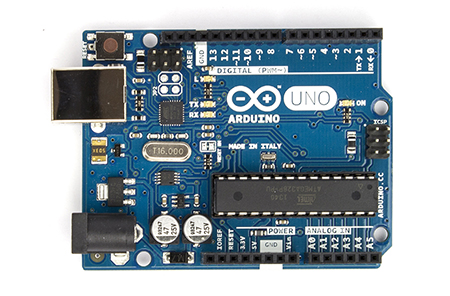
\includegraphics[width=0.5\textwidth]{chapters/analysis/figs/ArduinoUno.jpg}
\caption{The Arduino Uno board\cite{arduinointroduction}.}
\label{fig:arduinouno}
\end{figure}

\begin{center}

\begin{table}[]
	\centering
	\begin{tabular}{|l|c|c|}
		\hline
		\rowcolor[HTML]{C0C0C0} 
		Unit                        & Arduino Uno                       & Arduino Mega                     \\ \hline
		Microcontroller             & ATmega328                         & ATmega1280                       \\
		Operating Voltage           & \multicolumn{2}{c|}{5V}                                              \\
		Input Voltage (recommended) & \multicolumn{2}{c|}{7-12V}                                           \\
		Input Voltage (limits)      & \multicolumn{2}{c|}{6-20V}                                           \\
		Digital I/O Pins            & 14 (6 provide PWM output)         & 54 (15 provide PWM output)       \\
		Analog Input Pins           & 6                                 & 16                               \\
		DC Current per I/O Pin      & \multicolumn{2}{c|}{40 mA}                                           \\
		DC Current for 3.3V Pin     & \multicolumn{2}{c|}{50 mA}                                           \\
		Flash Memory                & 32 KB (0.5 KB used by bootloader) & 128 KB (4 KB used by bootloader) \\
		SRAM                        & 2 KB                              & 8 KB                                \\
		EEPROM                      & 1 KB                              & 4 KB                               \\
		Clock Speed                 & \multicolumn{2}{c|}{16 MHz}                                          \\ \hline
	\end{tabular}
	\caption{Arduino Uno and Mega specifications \cite{arduinouno}\cite{arduinomega}.}
\end{table}\label{tab:arduspecs}
\end{center}

\iffalse%udkommenteret
\begin{table}
\begin{tabular}{| l | l |}
\hline
Microcontroller & ATmega328\\
Operating Voltage & 5V\\
Input Voltage (recommended) & 7-12V\\
Input Voltage (limits) & 6-20V\\
Digital I/O Pins & 14 (of which 6 provide PWM output)\\
Analog Input Pins & 6\\
DC Current per I/O Pin & 40 mA\\
DC Current for 3.3V Pin & 50 mA\\
Flash Memory & 32 KB (ATmega328) of which 0.5 KB is used by bootloader\\
SRAM & 2 KB (ATmega328)\\
EEPROM & 1 KB (ATmega328)\\
Clock Speed & 16 MHz\\
\hline
\end{tabular}
\caption{Specifications for the Arduino Uno\cite{arduinouno}.}
\end{table}
\label{tab:unospec}
\fi

\textbf{Arduino Mega}\\
The Arduino Mega is a larger version of the Uno. The Mega has more memory and pins, which makes it better for handling larger programs or amounts of data. This also allows more components can be connected to the board. Since the clock speed is the same as the Uno, the Mega will not process data faster.

\begin{figure}[h!]
\centering
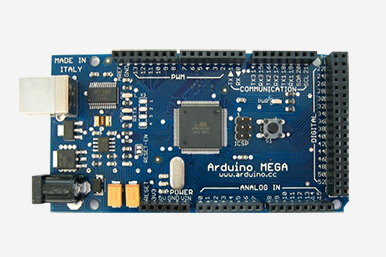
\includegraphics[width=0.6\textwidth]{chapters/analysis/figs/ArduinoMega.jpg}
\caption{The Arduino Mega board\cite{arduinomegaimg}.}
\label{fig:arduinomega}
\end{figure}

\iffalse%udkommenteret
\begin{table}[h!]
\begin{tabular}{| l | l |}
\hline
Microcontroller & ATmega1280\\
Operating Voltage & 5V\\
Input Voltage (recommended) & 7-12V\\
Input Voltage (limits) & 6-20V\\
Digital I/O Pins & 54 (of which 15 provide PWM output)\\
Analog Input Pins & 16\\
DC Current per I/O Pin & 40 mA\\
DC Current for 3.3V Pin & 50 mA\\
Flash Memory & 128 KB of which 4 KB used by bootloader\\
SRAM & 8 KB\\
EEPROM & 4 KB\\
Clock Speed & 16 MHz\\
\hline
\end{tabular}
\caption{Specifications for the Arduino Mega\cite{arduinomega}.}
\end{table}
\label{tab:megaspec}
\fi

Both Arduino Uno and Mega are used in this project, because having specifications good enough for the project and their availability to the project group. The Mega boards are not faster, but can contain more program code and allows for more components. This is not necessary\todo{how do you know this?}, but the devices are used as they were available\todo{FLYT TIL DESIGN}.

\subsection{Raspberry Pi}
Raspberry Pi is a series of single board computers. The Raspberry Pi is developed by the Raspberry Pi Foundation seated in the UK. The Raspberry Pi series contains some rather powerful controllers compared to their credit card sized boards, which makes them great as small processing units.

Something about those stupid pins....

Because of the power and memory of a Raspberry pi, a Linux OS is usually installed on a SD card and then plugged into the Pi for executing. A Raspberry Pi also contains a GPU, video output, and USB input.

In the following subsection a Raspberry Pi B+ will be described. The different models usually differs on CPU speed and memory, but a main difference from the early models is network connectivity.

\textbf{Raspberry Pi B+}\\
The Raspberry Pi B+ contains the specifications shown on \ref{tab:pibplusspec} along with HDMI video output and Ethernet connectivity. As main storage a micro SD card must be installed, which also contains the OS.

The Raspberry Pi B+ model is used in this project as the receiver and handler of data. This device has the capability to create user interfaces and show the data received from the sensors. The B+ model is used as it was available\todo{FLYT TIL DESIGN}.

\begin{figure}[h!]
\centering
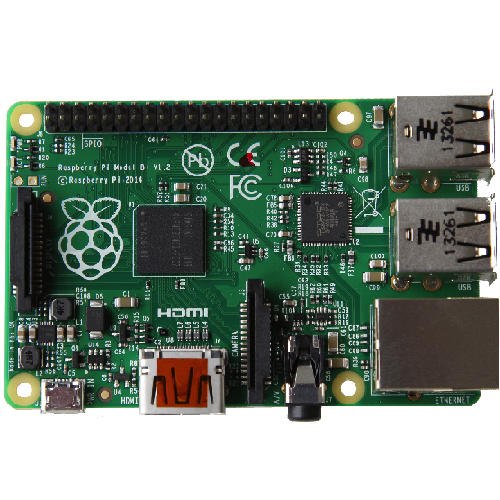
\includegraphics[width=0.6\textwidth]{chapters/analysis/figs/raspberry-pi-model-b-plus.png}
\caption{Raspberry Pi B+\cite{pibplus}.}
\label{fig:pibplus}
\end{figure}

\begin{table}[h!]
\centering
\begin{tabular}{| l | l |}
\hline
Microcontroller & Broadcom BCM2835\\
RAM & 512MB\\
Extended GPIO Pins & 40\\
USB Ports & 4\\
Clock Speed & 700 MHz\\
\hline
\end{tabular}
\caption{Specifications for Raspberry Pi B+\cite{pispecs}.}
\end{table}
\label{tab:pibplusspec}